\documentclass[11pt]{amsbook}

\usepackage{../HBSuerDemir}
\usepackage{graphicx}

\begin{document}

\hPage{b2p1/228 \footnote{please look at image source file for .svg files} \footnote{left paragraphs of the figures has no indent, i try many of way of adding figure(wrapfig...). This is the most efficient result.}\footnote{i use $\gamma$ for strange r}} 

\begin{exmp}
(Circular helix). Consider the curve
    \begin{align*}
        r(\theta) = a\cdot cos\theta \cdot i + a \cdot sin\theta \cdot j + b \cdot \theta \cdot k 
    \end{align*}
        \par or 
    \begin{align*}
        \gamma :  \left \{ \begin{array}{lr}
        x = a \cdot \cos\theta\\
        y = a \cdot \sin\theta\\
        z = b \cdot \theta
        \end{array}\right. \quad \text{(a$>$0, b$>$0),  $\theta_\epsilon$R.}
    \end{align*}
\begin{figure}[htbp]
\begin{minipage}{0.60\linewidth}
Elimination of $\theta$ between x, y gives the relation $x^2 + y^2 = a^2$ which is a right circular cylinder (a projecting cylinder). Hence $\gamma$ lies on this cylinder. $\theta$ varies, P($a\cdot \cos \theta$, $a\cdot \cos \theta$, b$\cdot \theta$) lying on this cylinder, describe curve called \underline{circular helix.} \\
That arc corresponding to the interval (0, 2$\pi$) is shown on the figure, starting at A(a, 0, 0) and ending at B(a, 0, 2$\pi$b). 
\end{minipage}
\begin{minipage}{0.35\linewidth}
    \centering
    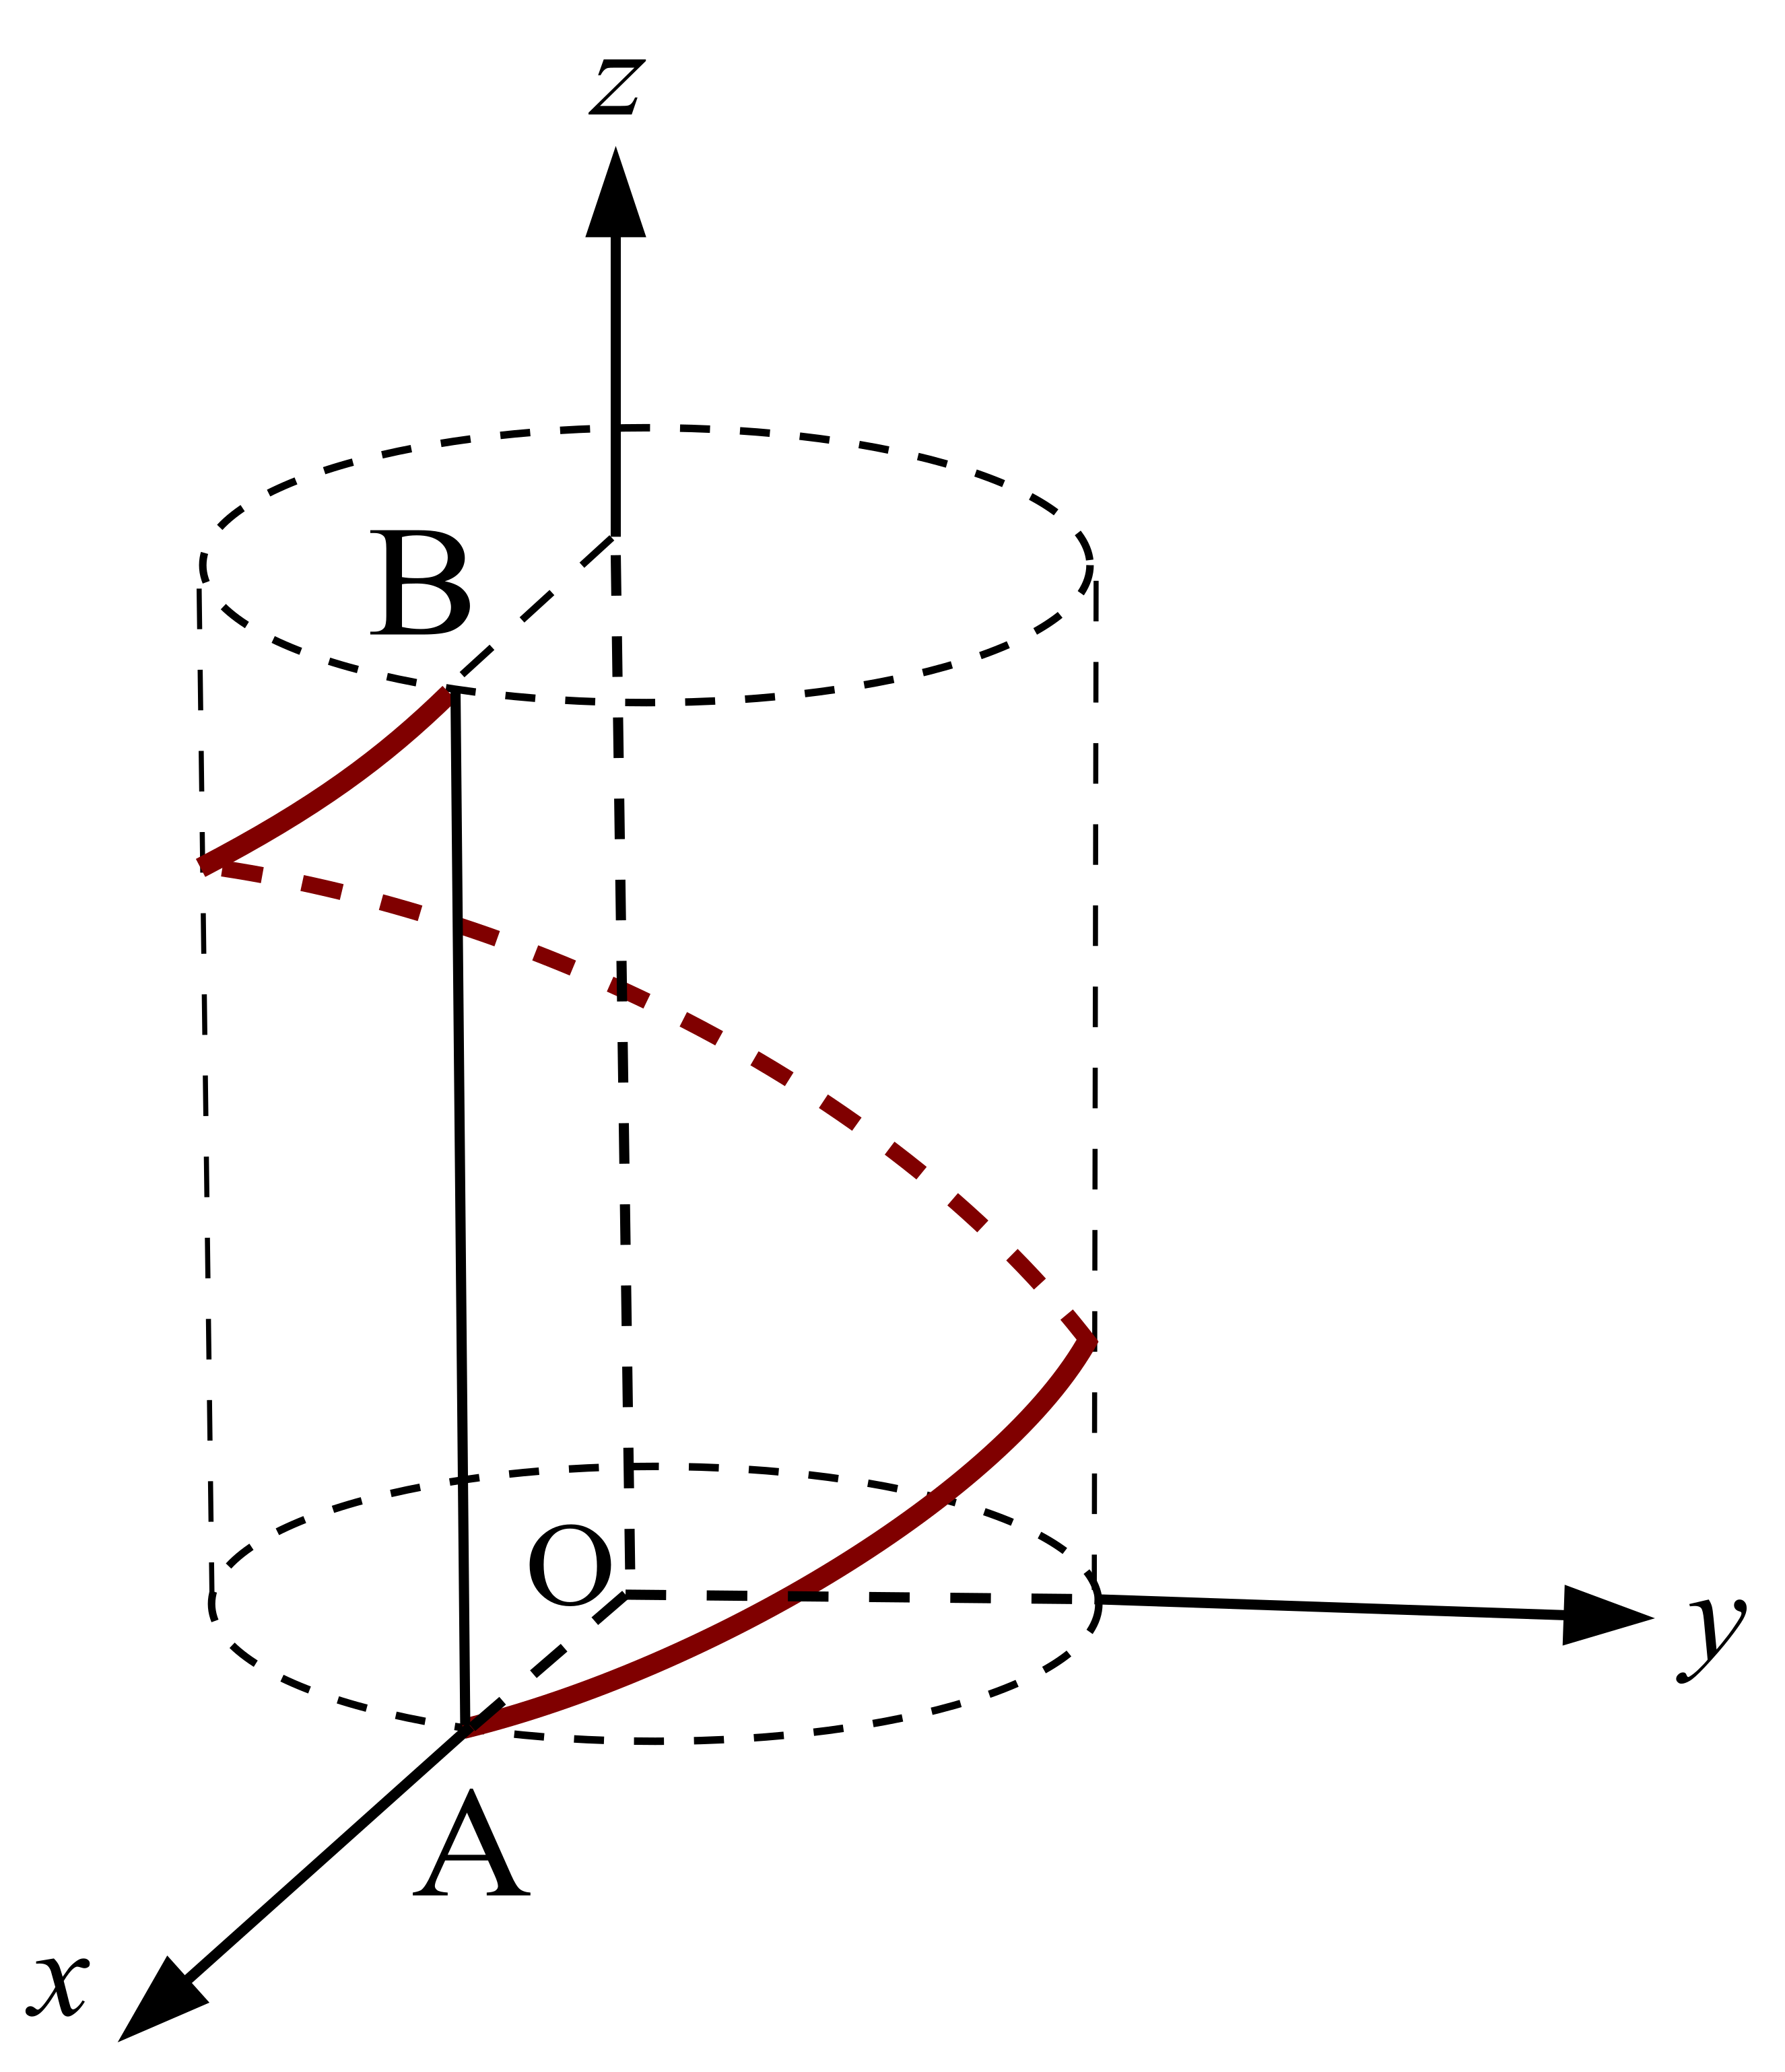
\includegraphics[width=0.85\linewidth]{images/helix.png} 
    \end{minipage}
\end{figure}
\par
The whole curve obtained by translating this arc in the direction of z-axis by multiplies of 2$\pi$b.
\begin{figure}[htbp]
\begin{minipage}{0.60\linewidth}
\par
    The circular helix has the property that when the cylinder is cut along the line AB (or the line $x=a$, $y=0$) and developed on a plane the curve becomes a line with slope $\frac{2\pi b}{2\pi a} = \frac{b}{a}$.
\end{minipage}
\begin{minipage}{0.35\linewidth}
    \centering
    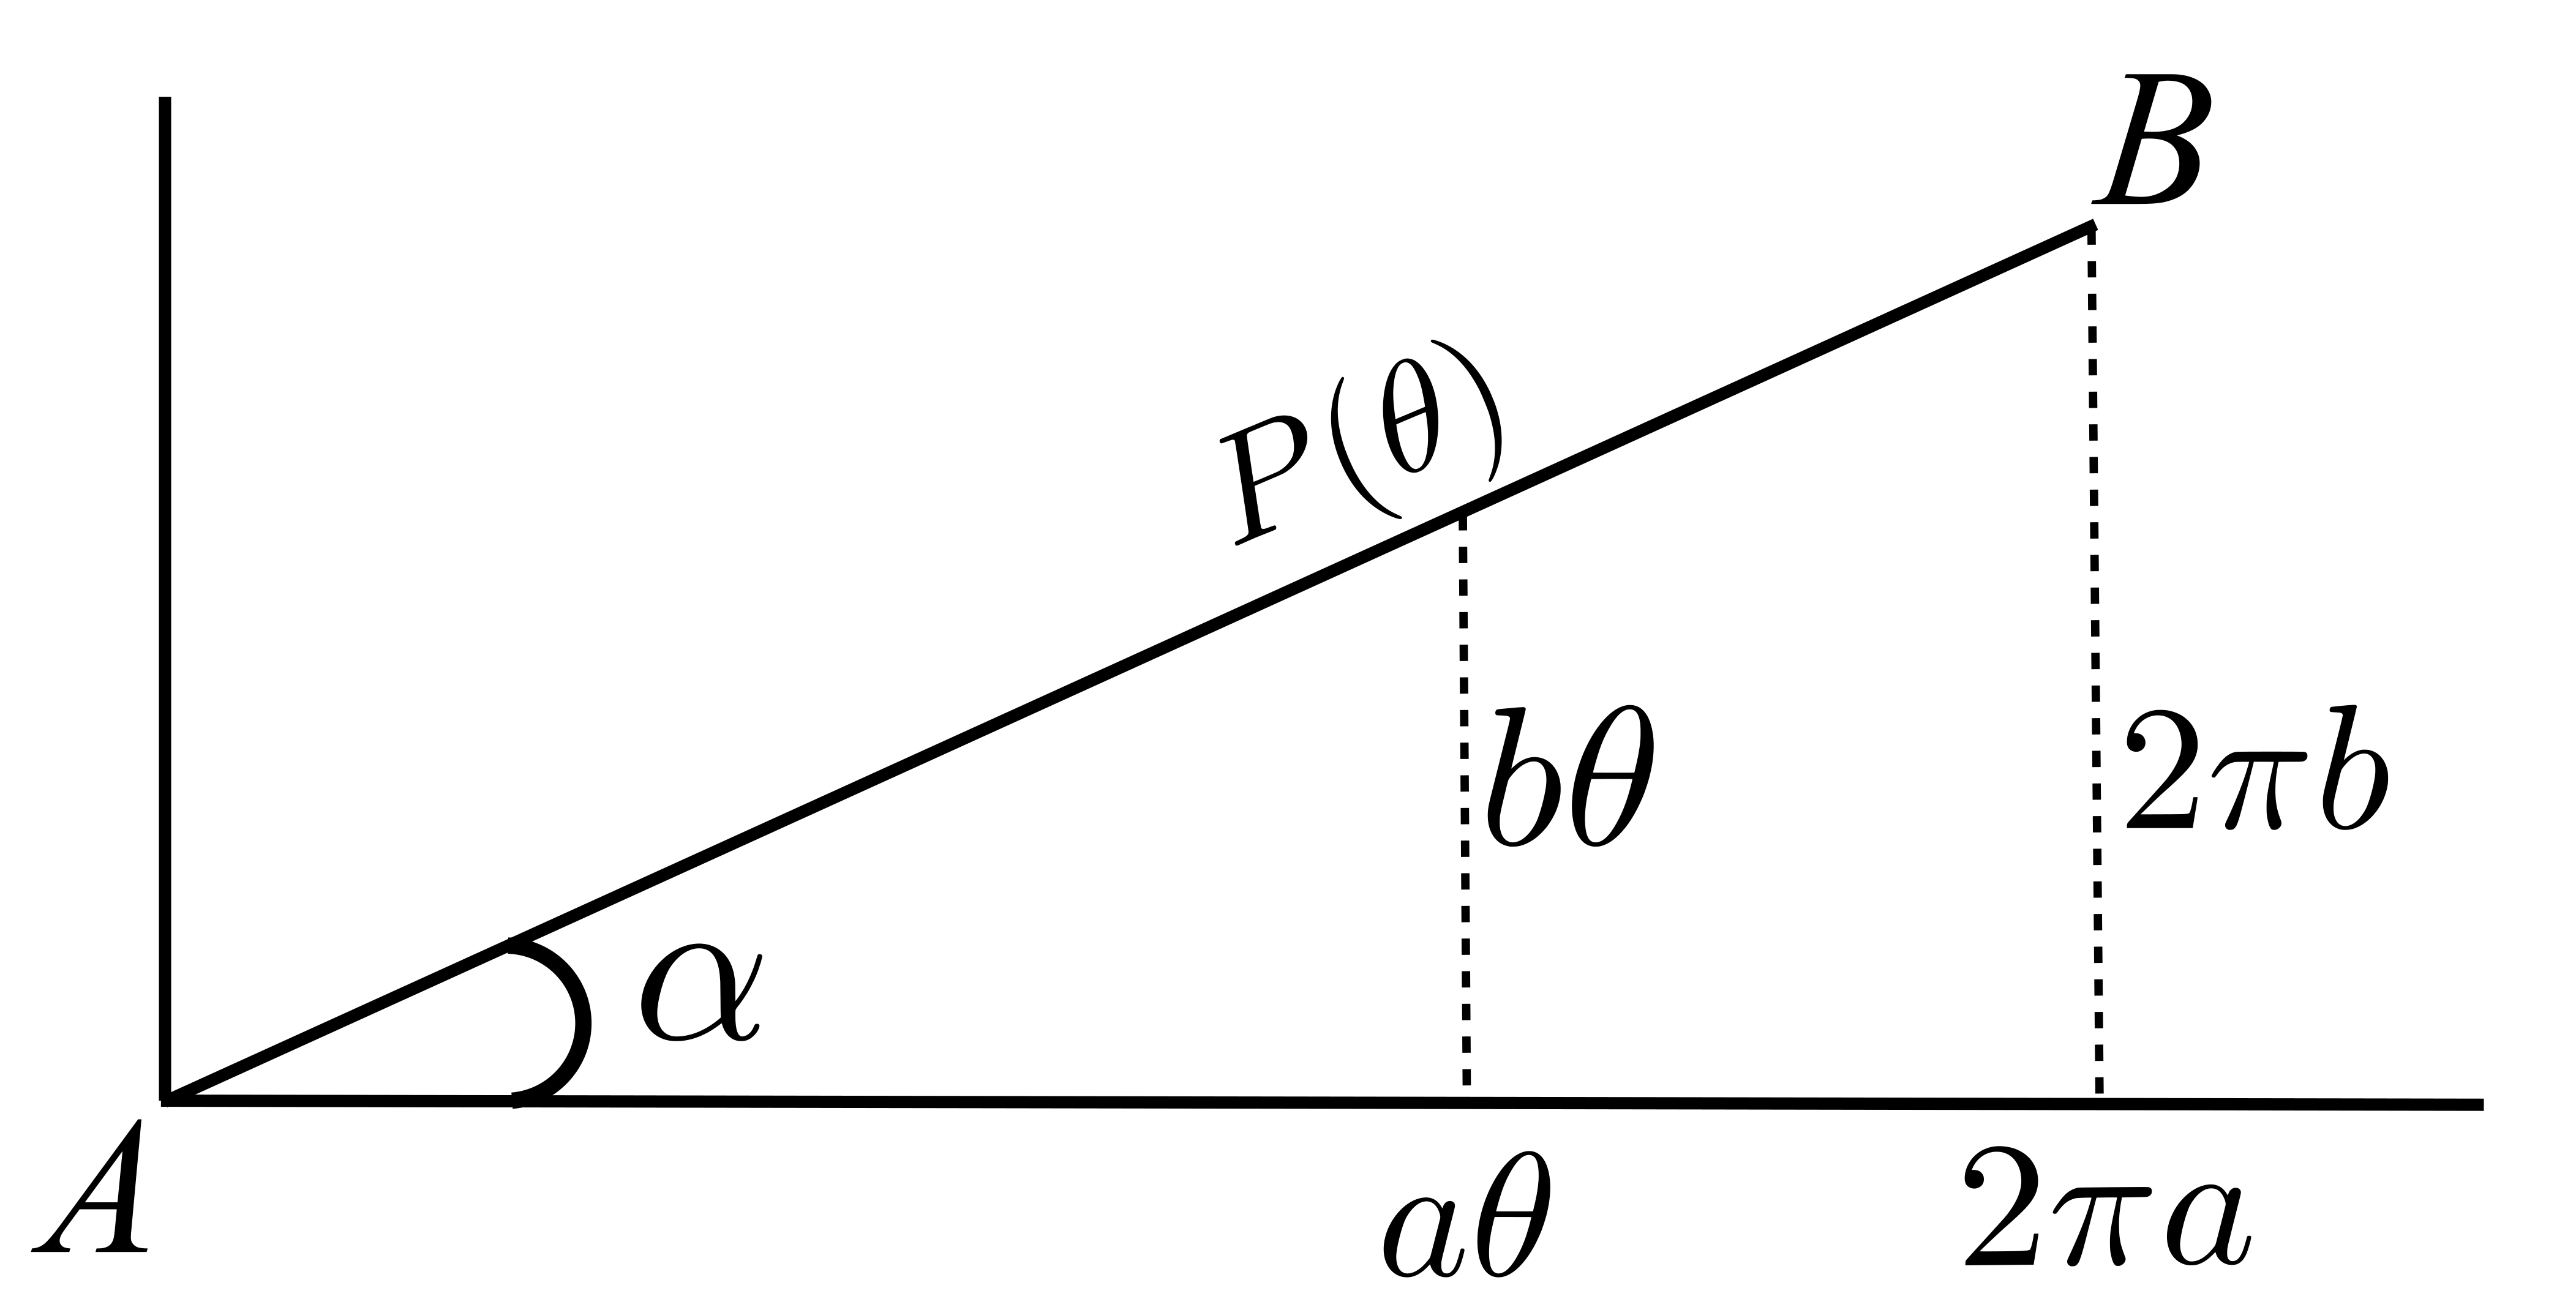
\includegraphics[width=0.95\linewidth]{images/middle.png} 
    \end{minipage}
\end{figure}
\end{exmp}
\underline{Geometric interpretation of r(t)} 
Let
\begin{align*}
    \gamma: r(t) = (x(t), y(t), z(t)), \quad t_\epsilon(\alpha, \; \beta)
\end{align*}
\begin{figure}[htbp]
\begin{minipage}{0.52\linewidth}
    be a space curve. Let the equation of the tangent line at $P_0(t_o)$ be desired. Consider a nearby point $P(t)$ on $\gamma$. The tangent line at $P_0$ is the limiting position of the line $P_0P$ as $P$ $\rightarrow$ $P_0$. The direction numbers
\end{minipage}
\begin{minipage}{0.45\linewidth}
    \centering
    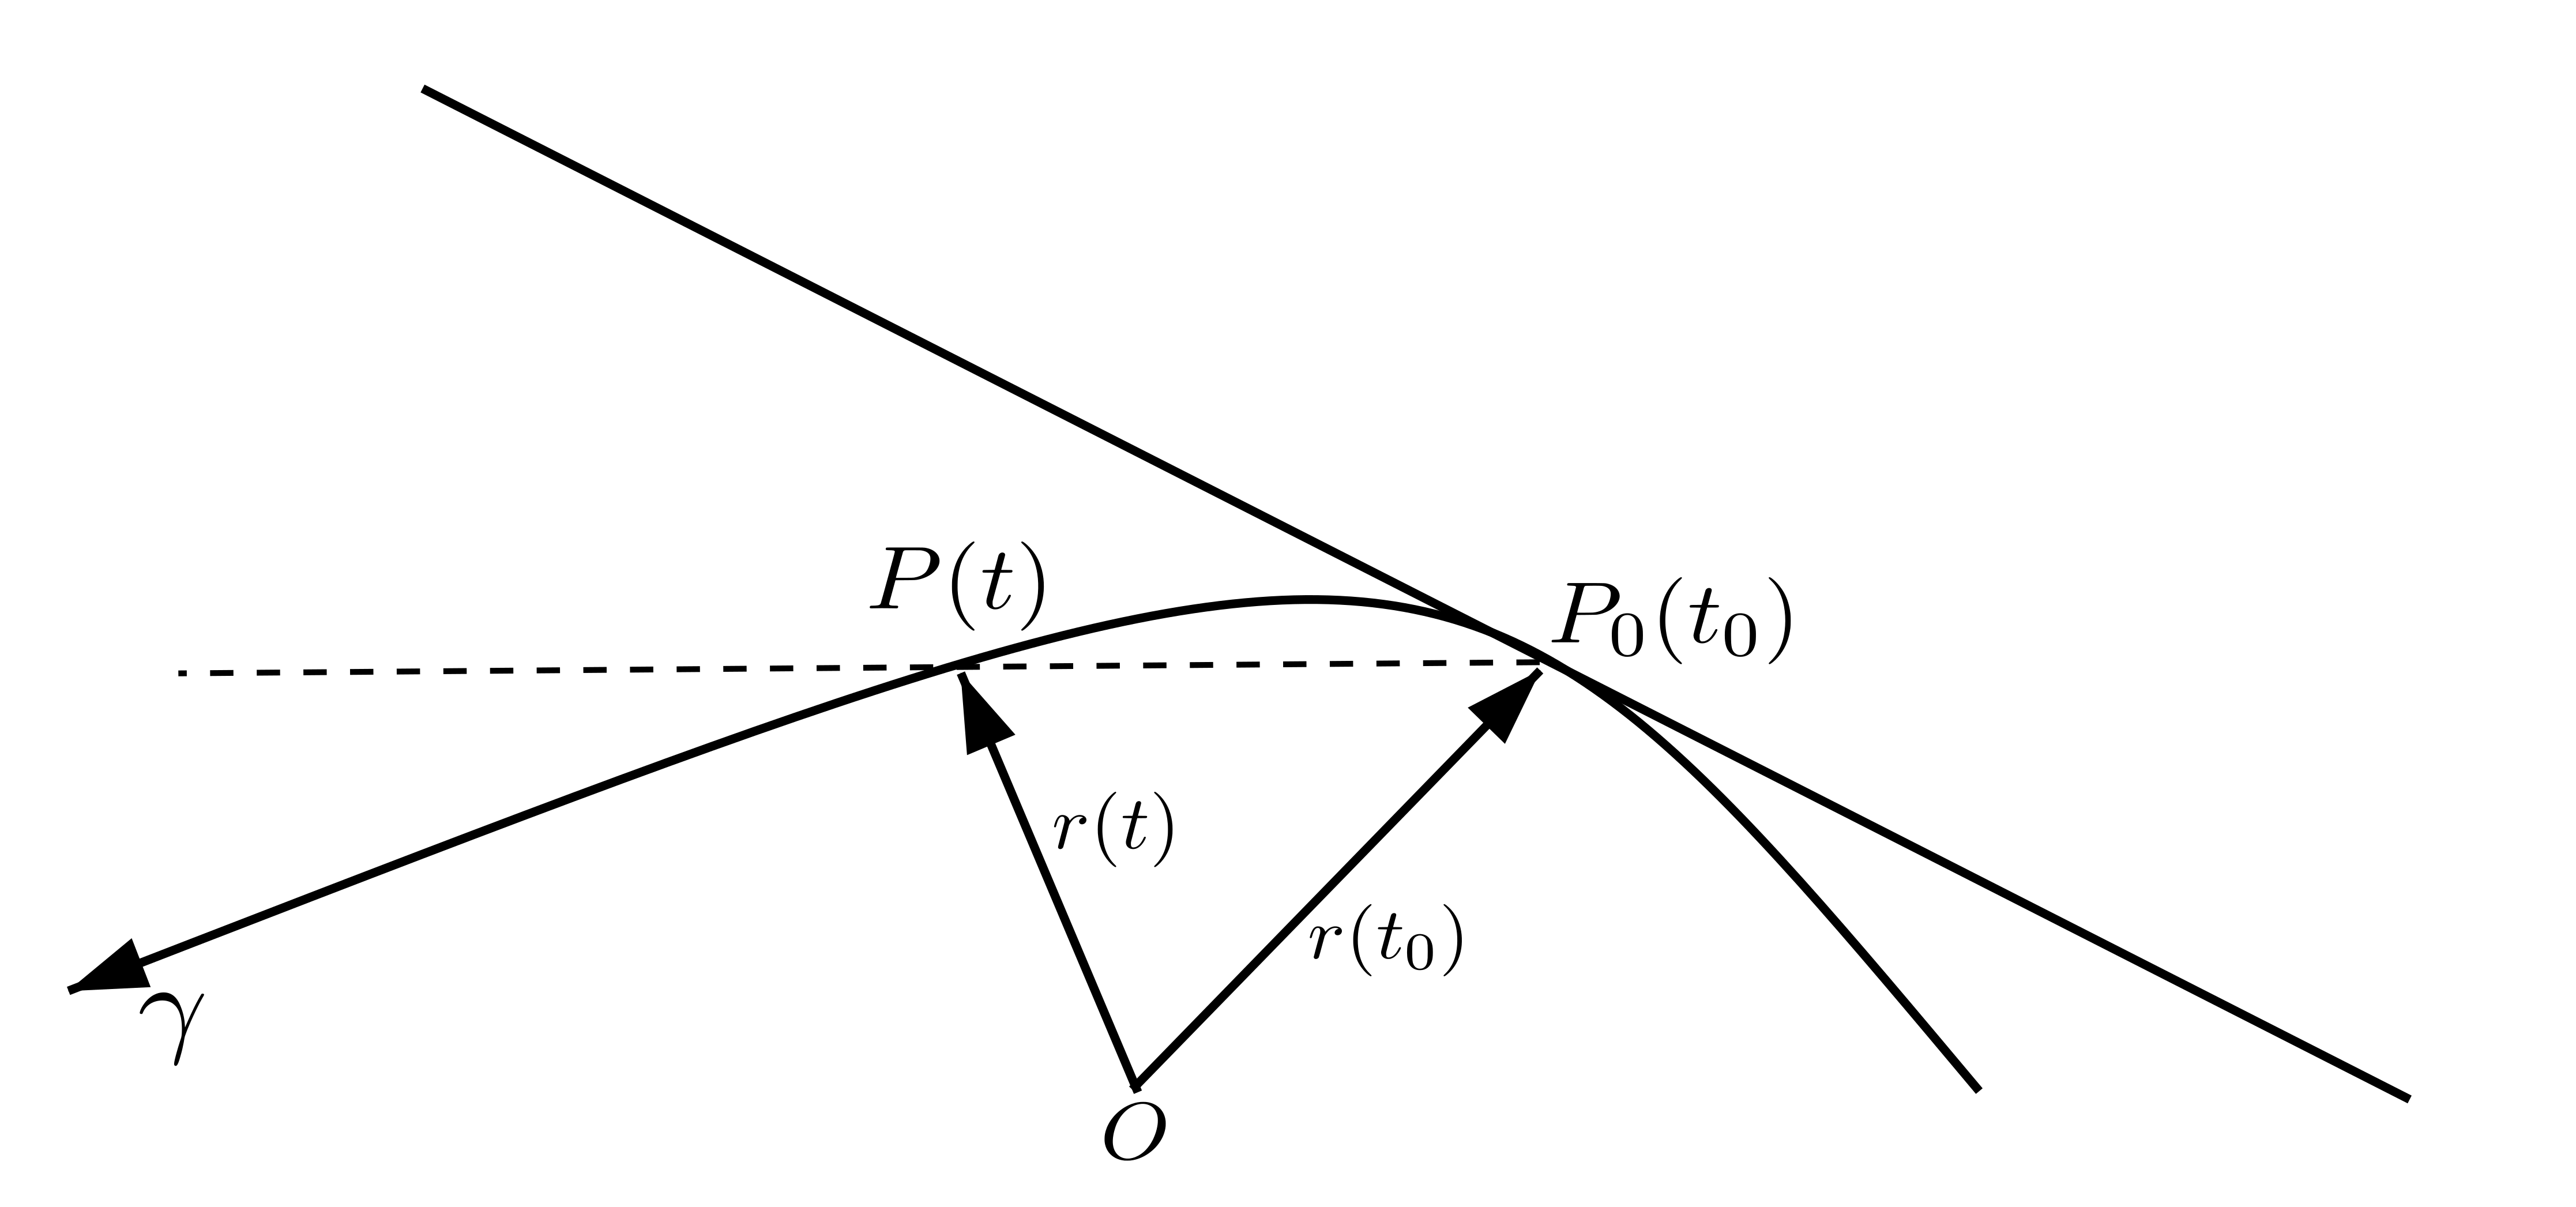
\includegraphics[width=1.35\linewidth]{images/last.png} 
    \end{minipage}
\end{figure}
\end{document}